\section{Technical Report}		
\subsection{Introduction and Summary}

The contents of this chapter correspond almost to the temporal line or chronology of the project. First we explain the \gls{opengl} concepts we learned and applied in the application, then we describe how we implemented the different file readers and the mathematics behind the movement calculation. After that we continue with the research process we followed in order to improve the accuracy of the movement displayed. Out of this time line are the tests, dependencies and the code statistics, besides of the results.


\subsection{OpenGL} \label{opengl}

\subsubsection{Introduction}

By definition, \gls{opengl} is a graphics API which provides an abstraction layer between the application and the underlying graphics subsystem. 
The commands \cite{superbible} from the program are taken by OpenGL and sent to the underlying graphics hardware, which works on them in an efficient manner to produce the desired result as quickly and efficiently as possible.

There could be many commands lined up to execute on the hardware, and some may even be partially completed. This allows their execution to be overlapped in such a way that one command might run concurrently with an earlier stage of another. Furthermore, computer graphics generally consists of many repetitions of very similar tasks, and these tasks are usually independent of one another. For example, the result of colouring one pixel does not necessarily depend on any other. Just like a car plant can build multiple cars simultaneously, OpenGL can break up the work you give it and work on its fundamental elements in parallel. \hl{"Through a combination of pipelining and parallelism, incredible performance of modern graphics processors is realized"} \cite{superbible}.

This \emph{abstraction layer} \cite{superbible} removes the necessity of knowing who made the graphics processor (or graphics processing unit [GPU]), how it works, or how well it performs for the application as well as its developer. It remains possible to determine this information, but the point is that you should not need to.

\subsubsubsection{Core and Compatibility Profiles} \label{opengl-profiles}

Since the first OpenGL version in 1992 \cite{superbible} the graphics hardware and software have continuously evolved at a fast pace. Over time, the price of graphics hardware came down, performance went up, and new features showed up in affordable graphics processors and were added to OpenGL. Most of these features originated in extensions proposed by members of the \gls{gls-arb}. Some interacted well with each other and with existing features in OpenGL, and some did not. 

For many years, the \gls{ARB} held a strong position on backward compatibility, as it still does today. However, this backward compatibility comes at a significant cost. 
For these and other reasons, in 2008, the ARB decided it would "fork" the OpenGL specification into two profiles. 

The first is the modern, \textbf{core profile}, which removes a number of legacy features, leaving only those that are truly accelerated by current graphics hardware. This specification is several hundred pages shorter than the compatibility profile. On top of that, on some platforms, newer features are available only if you are using the core profile of OpenGL.

The \textbf{compatibility profile} maintains backward compatibility with all revisions of OpenGL back to version 1.0. As a consequence, software written in 1992 should compile and run on a modern graphics card with a thousand times greater performance today than when that program was first produced.

This project is developed in the core profile, with OpenGL version 3.3. As of today, much higher versions of OpenGL have been released (at the time of writing 4.5). 
The answer to the logical question of why we used OpenGL 3.3 when version 4.5 is out, is that all future versions of OpenGL starting from 3.3 mainly just add additional features to OpenGL without changing the core mechanics; the newer versions just introduce slightly more efficient or more useful ways to accomplish the same tasks or support the latest graphics cards. As a result, all concepts and techniques remain the same within modern OpenGL versions and it is perfectly valid to learn and use OpenGL 3.3 and thereby supporting as many graphics processors as possible \cite{learnopengl}.

\subsubsubsection{Recommended definitions}

For a better comprehension of the following sections, we recommend to consult the following terms in the glossary:
\begin{itemize}
	\item \textbf{\Gls{vertex}}
	\item \textbf{\Gls{primitive}}
	\item \textbf{\Gls{shader}} (Extended explanations of this term follow below)
	\item \textbf{\gls{object-space} or \gls{model-space}}
	\item \textbf{\gls{world-space}}
	\item \textbf{\gls{view-space}}
	\item \textbf{\gls{clip-space}}
	\item \textbf{\gls{window-space}}
\end{itemize}


\subsubsection{Graphics Pipeline} \label{graphis-pipeline}
Current graphics processing units (GPUs) consist of large numbers of small programmable processors called shader cores, which run mini-programs called \glspl{shader}. Each core has a relatively low throughput, processing a single instruction of the shader in one or more clock cycles and normally lacking advanced features such as out-of-order execution, branch prediction, super-scalar issues, and so on.

 However, each GPU might contain anywhere from a few tens to a few thousands of these cores, and together they can perform an immense amount of work. \hl{"The graphics system is broken into a number of stages, each represented either by a shader or by a fixed-function, possibly configurable processing block"} \cite{superbible}. Figure \ref{fig:graphics_pipeline_simple} shows a simplified schematic of the graphics pipeline.

\begin{figure}[h!]
	\centering
	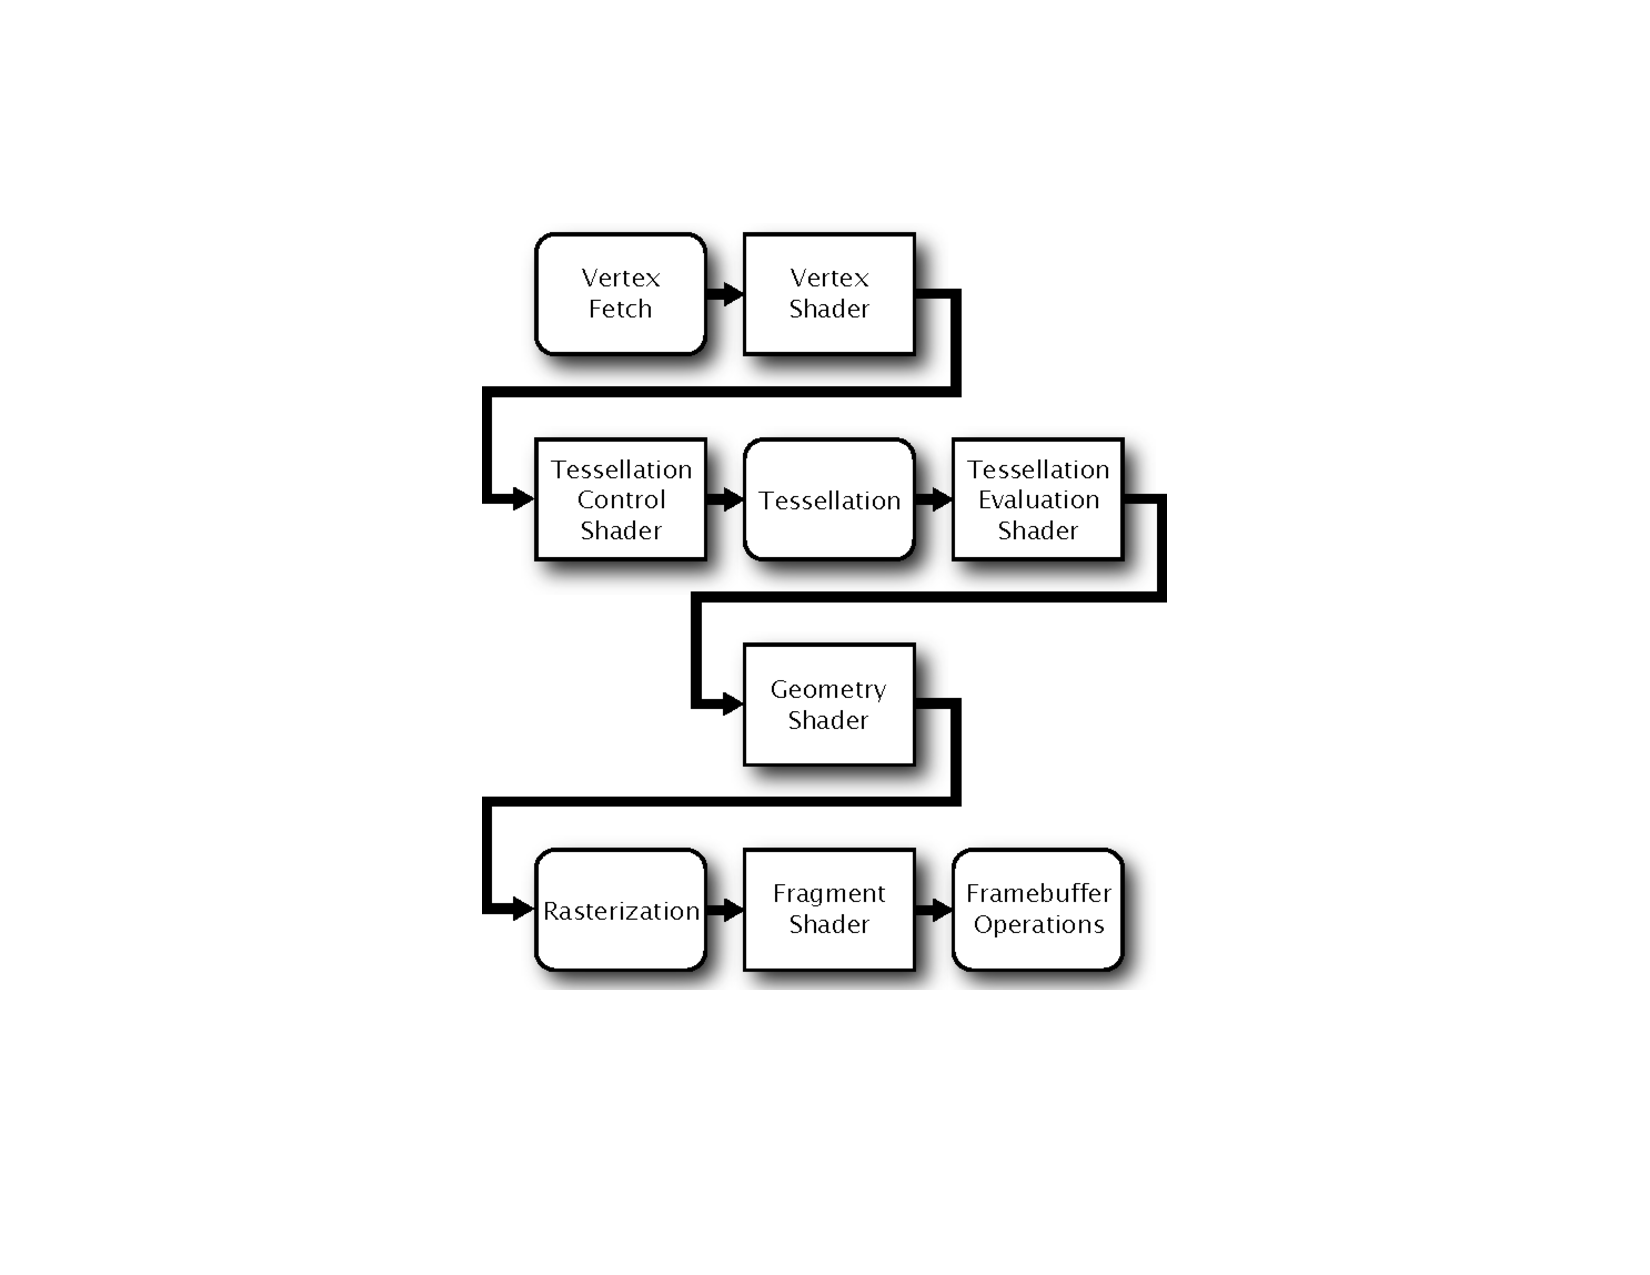
\includegraphics[width=0.3\textwidth]{graphics_pipeline_simple}
	\caption{Simplified graphics pipeline \cite{superbible}}
	\label{fig:graphics_pipeline_simple}
\end{figure}

In the figure above, the boxes with rounded corners are considered fixed-function stages, whereas the boxes with square corners are programmable since they can execute \glspl{shader} that you developed.

In the vertex fetch stage, we pass in a collection of \glspl{vertex} or \gls{vertex} data as input to the graphics pipeline. These \glspl{vertex} grouped by three should form a triangle.

The first part of the pipeline is the \gls{vertex-shader} that takes a single \gls{vertex} as input. The main purpose of the  \gls{vertex-shader} is to transform \gls{vertex} coordinates into \gls{gls-normalized-device-coordinates}. It also allows us to do some basic processing on the vertex attributes.

In the primitive assembly stage or \gls{tessellation}, the \gls{tessellation-control-shader} takes all the \glspl{vertex} from the \gls{vertex-shader} and assembles all the point(s) to the \gls{primitive} shape given - a triangle for example.

The output of the primitive assembly stage is passed to the \gls{geometry-shader}. The \gls{geometry-shader} takes a collection of vertices that form a \gls{primitive} and has the ability to generate other shapes by emitting new vertices to form new (more of the same or even other) \gls{primitive}(s). 

The output of the \gls{geometry-shader} is then passed on to the rasterization stage, where it maps the resulting \gls{primitive}(s) to the corresponding pixels on the final screen (2D), resulting in fragments for the \gls{fragment-shader} to use. Before the \gls{fragment-shader} runs, clipping is performed. Clipping discards all fragments located outside of the viewing perspective fitting the screen, resulting in a better performance.

The main purpose of the \gls{fragment-shader} is to calculate the final colour of a pixel and this is usually the stage where all the advanced \gls{opengl} effects occur. The \gls{fragment-shader} contains data about the 3D scene that it can use to calculate the final pixel colours (e.g. lights, shadows, colour of the light, reflections and so on).

After all the corresponding colour values have been determined, the final object will then pass through one more stage called the alpha test \cite{alphatest} and blending stage \cite{blendtest}. This stage checks the corresponding depth (and stencil) value of the fragment and uses those to check if the resulting fragment is in front or behind other objects and should be discarded accordingly. The stage also checks for alpha values (alpha values define the opacity of an object) and blends the objects as necessary. So even if a pixel output colour is calculated in the \gls{fragment-shader}, the final pixel colour could still be something entirely different when rendering multiple \glspl{primitive}.

In the figure \ref{fig:graphics_pipeline} below we can now observe the graphics pipeline with a short description of what each \gls{shader} does at its corresponding stage.

\begin{figure}[h!]
	\centering
	\caption{Extended graphics pipeline \cite{learnopengl}}
	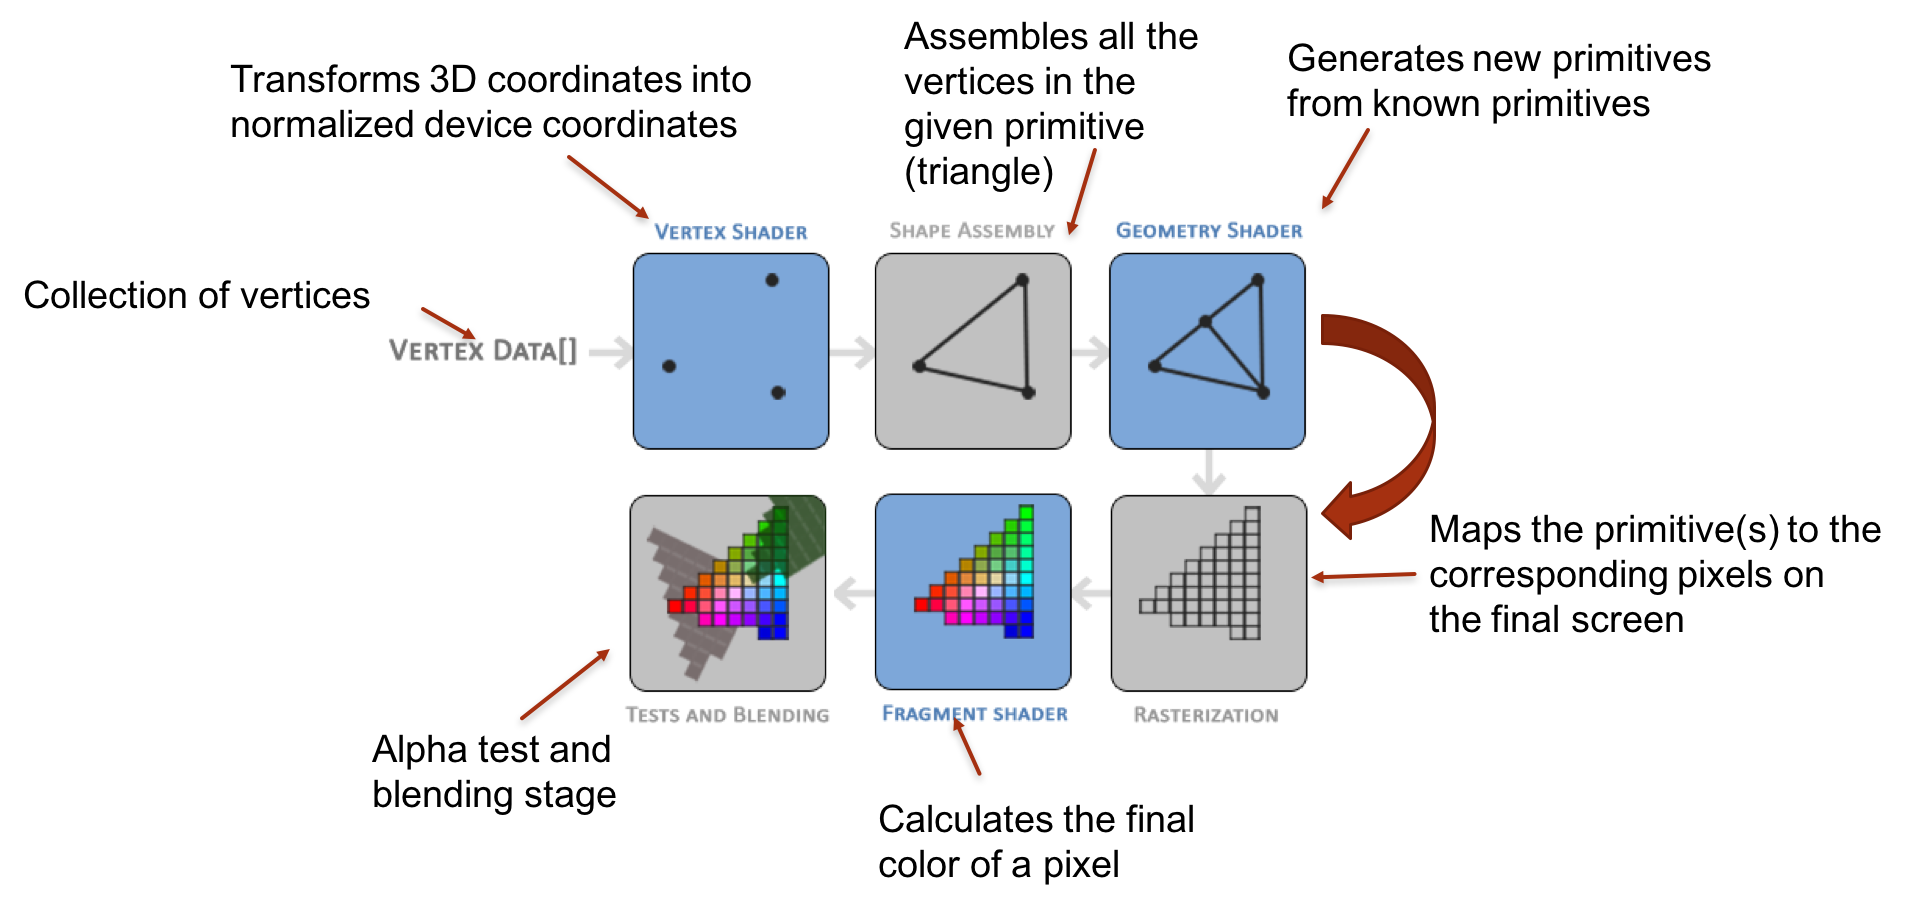
\includegraphics[width=0.9\textwidth]{graphics_pipeline}	
	\label{fig:graphics_pipeline}
\end{figure}

\newpage
\subsubsection{Shaders}

\hl{"\glspl{shader} are little programs that rest on the graphics processing unit (GPU) and transform inputs to outputs. They usually form a chain in which the output of a first shader serves as input of the following shader."} \cite{shading}

Each \gls{shader} executes in a different section of the OpenGL pipeline. All \glspl{shader} are executed on the GPU, and as the name implies, they (typically) implement the algorithms related to the lighting and shading effects of an image. However, \glspl{shader} are capable of doing much more than just implementing a shading algorithm. They are also capable of performing animation, tessellation, or even generalized computation.

OpenGL \glspl{shader} are written in the \gls{glsl} (GLSL). This language has its origins in C, but has been modified over time to make it better suited to be run on graphics processors, containing features targeted at vector and matrix manipulation. The compiler for this language is built into OpenGL. 

The source code for a \gls{shader} is placed into a \emph{shader object} and compiled. Multiple shader objects can then be linked together to form a \emph{program object}. Each program object can contain \glspl{shader} for one or more shader stages. The shader stages of OpenGL are \glspl{vertex-shader}, \glspl{tessellation-control-shader} and evaluation shaders, \glspl{geometry-shader}, \glspl{fragment-shader}, as well as compute shaders. 


\subsubsection{Shaders Syntax}

The goal of this section is to provide a short introduction to the \gls{glsl} and \gls{shader} syntax. For deeper comprehension please refer to the \hl{\emph{OpenGL 4 Shading Language Cookbook}} \cite{shading}.

\glspl{shader} always begin with a version declaration, followed by the main function as well as an optional list of input and output variables, uniforms \cite{learnopengl}:
\begin{lstlisting}[language=C++, caption=Vertex Shader syntax \cite{shading}]
#version version_number

in type in_variable_name;
in type in_variable_name;

out type out_variable_name;

uniform type uniform_name;

void main() {
	// Process input(s) and do some weird graphics stuff
	//...
	// Output processed stuff to output variable
	out_variable_name = weird_stuff_we_processed;
}
\end{lstlisting}

\subsubsection{Vertex attributes and its number in a vertex shader}

In \gls{GLSL}, the mechanism for getting data in and out of \glspl{shader} is declaring global variables with the \verb|in| and \verb|out| storage qualifiers \cite{superbible}. 

At the start of the OpenGL pipeline, the \verb|in| keyword is used to bring inputs into the \gls{vertex-shader}. Between stages, \verb|in| and \verb|out| can be used to form conduits from shader to shader and pass data between them.

The declaration of a variable with the \verb|in| storage qualifier marks the variable as an input to the \gls{vertex-shader}, which means that it is essentially an input to the OpenGL graphics pipeline. It is automatically filled in by the fixed-function vertex fetch stage. The variable becomes known as a \emph{vertex attribute} \cite{shading}.

Vertex attributes are how vertex data is introduced into the OpenGL pipeline. To declare a vertex attribute, you declare a variable in the \gls{vertex-shader} using the \verb|in| storage qualifier. 

The hardware limits the maximum number of vertex attributes. In OpenGL there are always at least 16 4-component vertex attributes. \cite{learnopengl}

\subsubsection{Ins and Outs}

In order to send data from one \gls{shader} to another it is necessary to declare an output in the sending shader and a similar input in the receiving shader. When the types and the names are equal on both sides OpenGL will link those variables together and then it's possible to send data between shaders.

In the code examples below a \verb|vertexColor| variable as a \verb|vec4| output is set in the (Listing \ref{code:vertex-shader}) vertex shader and a similar \verb|vertexColor| input variable is declared in the (Listing \ref{code:fragment-shader}) fragment shader. Since they both have the same type and name, the \verb|vertexColor| in the \gls{fragment-shader} is linked to the \verb|vertexColor| in the \gls{vertex-shader}. 

Because the colour is set to a dark-red color in the \gls{vertex-shader}, the resulting fragments should be dark-red as well. However, without the output colour specification in the \gls{fragment-shader}, OpenGL would render the object black or white \cite{learnopengl}.


\begin{lstlisting}[language=C++, caption={Vertex Shader}, label={code:vertex-shader}]
#version 450 core
layout (location = 0) in vec3 position;//The position variable has attribute position 0

out vec4 vertexColor; // Specify a color output to the fragment shader

void main() {
 gl_Position = vec4(position, 1.0); //We give directly a vec3 to vec4's constructor
 vertexColor = vec4(0.5f, 0.0f, 0.0f, 1.0f);//Set the output variable to a dark-red color
}

\end{lstlisting}

\begin{lstlisting}[language=C++, caption={Fragment Shader}, label={code:fragment-shader}]
#version 450 core
in vec4 vertexColor; // The input variable from the vertex shader 
					 //(same name and same type)
out vec4 color; // the output color variable

void main() {
	color = vertexColor;
} 
\end{lstlisting}

\subsubsection{Uniforms}

Uniforms are another way to pass data from the application on the CPU to the \glspl{shader} on the graphics processing unit (GPU), but uniforms are slightly different compared to vertex attributes \cite{learnopengl}
\begin{itemize}
	\item Uniforms are \textbf{global}. A uniform variable is unique per shader program object, and can be accessed from any shader at any stage in the shader program
	\item Uniforms keep their values until they are reset or updated
\end{itemize}

Making a uniform is as simple as placing the keyword \verb|uniform| at the beginning of the variable declaration:
\begin{lstlisting}[language=C++, caption={Uniform}, label={code:uniform}]

#version 450 core
out vec4 FragColor; // Since uniforms are global variables, we can define them in 
					//any shader we'd like so no need to go through the vertex 
					//shader again to get something to the fragment shader.

uniform vec4 ourColor; // we set this variable in the OpenGL code.

void main() {
	FragColor = ourColor;
} 
\end{lstlisting}

\subsubsection{Using uniforms}

The uniform in the example above (Listing \ref{code:uniform}) is still empty. In order to fill it, it is necessary to find the index / location of the uniform attribute in the respective \gls{shader} in order to update its values. In the following example, we change the colour of a triangle gradually over time \cite{learnopengl}:

\begin{lstlisting}[language=C++, caption={Using uniforms}, label={code:uniform-usage}]

GLfloat timeValue = glfwGetTime();	// retrieve the running time in seconds
GLfloat greenValue = (sin(timeValue)/2) + 0.5;//vary the color in the range of 0.0 - 1.0

// query for the location of the ourColor uniform
GLint vertexColorLocation = glGetUniformLocation(shaderProgram, "ourColor"); 
glUseProgram(shaderProgram); //updating a uniform requires to first use the program
glUniform4f(vertexColorLocation, 0.0f, greenValue, 0.0f, 1.0f);// set the uniform value
\end{lstlisting}

Once the uniform values have been set, we can use them for rendering:
\begin{lstlisting}[language=C++, caption={Using uniforms for rendering}, label={code:uniform-rendering}]
//Changing the color gradually updating the uniform each render iteration
while(!glfwWindowShouldClose(window)) {
	// Check and call events
	glfwPollEvents();

	// Render
	// Clear the colorbuffer
	glClearColor(0.2f, 0.3f, 0.3f, 1.0f);
	glClear(GL_COLOR_BUFFER_BIT);
	
	// Be sure to activate the shader
	glUseProgram(shaderProgram);
	
	// Update the uniform color
	GLfloat timeValue = glfwGetTime();
	GLfloat greenValue = (sin(timeValue) / 2) + 0.5;
	GLint vertexColorLocation = glGetUniformLocation(shaderProgram, "ourColor");
	glUniform4f(vertexColorLocation, 0.0f, greenValue, 0.0f, 1.0f);
	
	// Now draw the triangle
	glBindVertexArray(VAO);
	glDrawArrays(GL_TRIANGLES, 0, 3);
	glBindVertexArray(0);
}
\end{lstlisting}

Resulting in: 
\begin{figure}[h!]
	\centering
	
\includegraphics[width=0.45\textwidth]{gradually_color}
	\caption{Uniform usage result \cite{learnopengl}}
	\label{fig:uniform-usage}
\end{figure}


\subsubsection{Model Space, World Space, Matrices and Transformations}

After describing the basics of \gls{opengl} and its building blocks, the \glspl{shader}, we continue with the different coordinates spaces and transformations used to finally display the graphics on the screen.

OpenGL expects all the \glspl{vertex} we want to become visible, to be in \gls{gls-normalized-device-coordinates} after each vertex shader run; coordinates outside this range will be clipped and therefore not be visible. These \gls{NDC} coordinates are then given to the rasterizer to transform them to 2D coordinates/pixels on a screen \cite{learnopengl}.

Transforming vertex coordinates to \gls{NDC} and then to screen coordinates is usually accomplished in a step-by-step fashion where we transform an object's vertices to several coordinate systems before finally transforming them to screen coordinates. The most popular transformations are referred to as model, view and projection.

The coordinate systems commonly used in 3D computer graphics are:
\begin{itemize}
	\item \textbf{\gls{object-space} or \gls{model-space}}
	\item \textbf{\gls{world-space}}
	\item \textbf{\gls{view-space}}
	\item \textbf{\gls{clip-space}}
\end{itemize}
In this section, we examine each of the coordinate spaces, and the transforms used to move vectors between them.

\subsubsection{Object Space}

\emph{Object coordinates}, \emph{Model Space} or \emph{Local Space}. The positions of \glspl{vertex} are interpreted relative to a local origin. Consider a cube as model. The origin of the model would probably be the centre of gravity or one of the vertices (corners) of the cube, $(0,0,0)$ for example. The origin is often the point used to rotate the model to place it into a new orientation \cite{superbible}.


\subsubsection{World Space and Model Matrix}

\hl{"This is where coordinates are stored relative to a fixed, global origin"} \cite{superbible}.
This is the coordinate space where you want your objects transformed to in such a way that they are all arranged within one place (preferably in a realistic fashion). The coordinates of your objects are transformed from model to world space using the \textbf{model matrix}.

\subsubsubsection{Model Matrix} \label{model-matrix}

\hl{"The model matrix is a transformation matrix that translates, scales and/or rotates your object to place it in the world space at a location/orientation they belong to"} \cite{learnopengl}. 
\begin{figure}[h!]
	\centering
	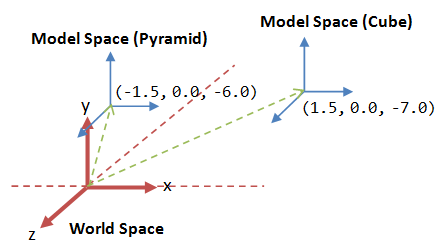
\includegraphics[width=0.45\textwidth]{worlds}
	\caption{Model and World Spaces \cite{3dgraphics}}
	\label{fig:world-model-space}
\end{figure}

\subsubsection{View Space and View Matrix} \label{view-matrix}

\emph{View Coordinates}, \emph{Eye Space} or often simply \emph{Camera}. View coordinates are relative to the position of the observer (hence the terms "camera" or "eye space") regardless of any transformations that may occur; you can think of them as "absolute" coordinates \cite{superbible}.

The view space is the result of transforming the world space coordinates to coordinates that are in front of the user's view. These transformations are generally stored inside the so called \textbf{view matrix}.

\begin{figure}[h!]
	\centering
	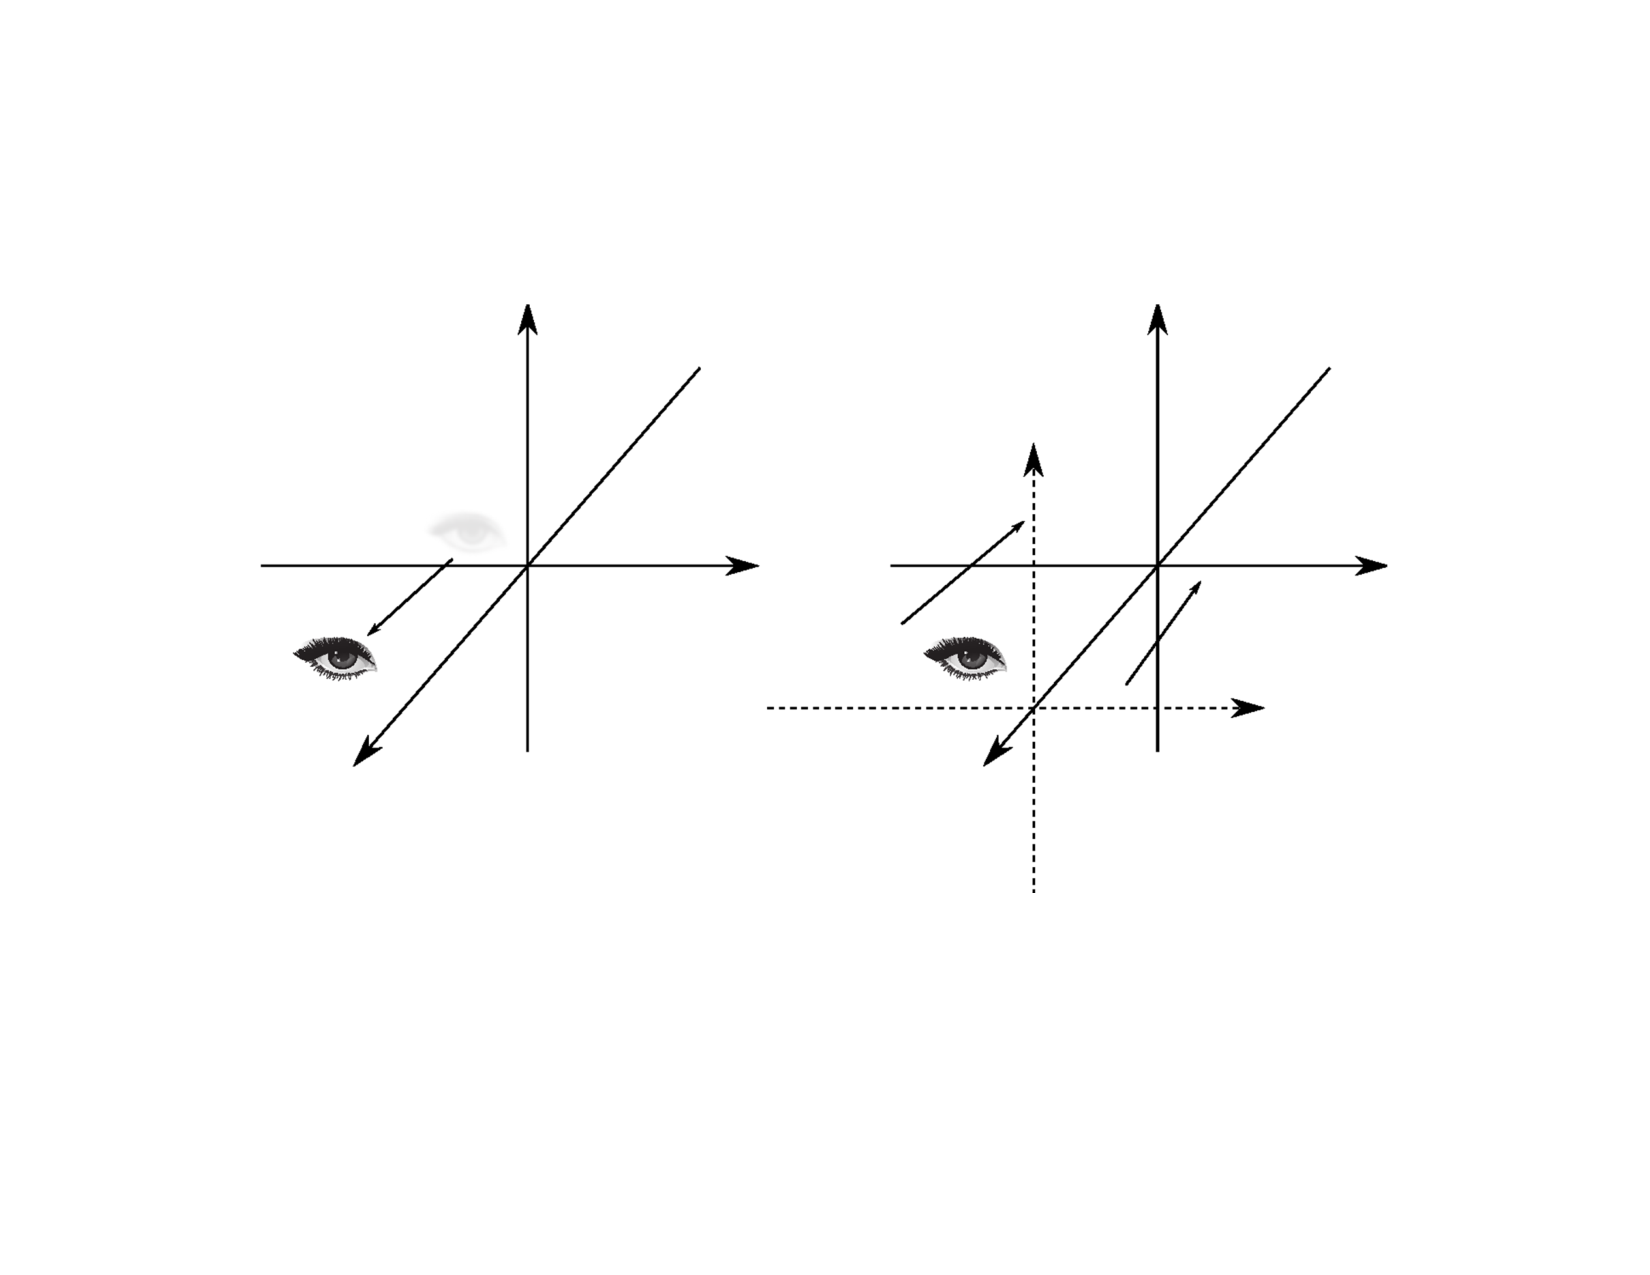
\includegraphics[width=0.4\textwidth]{view_space}
	\caption{Two perspectives of View Coordinates \cite{superbible}}
	\label{fig:view-space}
\end{figure}

\subsubsection{Clip Space and Projection Matrix}

\emph{Clipping} is an action consisting in discard coordinates which are not in a specified range. The remaining coordinates will end up as visible fragments on the screen. Therefore, the \emph{Clip Space} is the space within which the coordinates are eventually displayed on the screen:

\begin{figure}[h!]
	\centering
	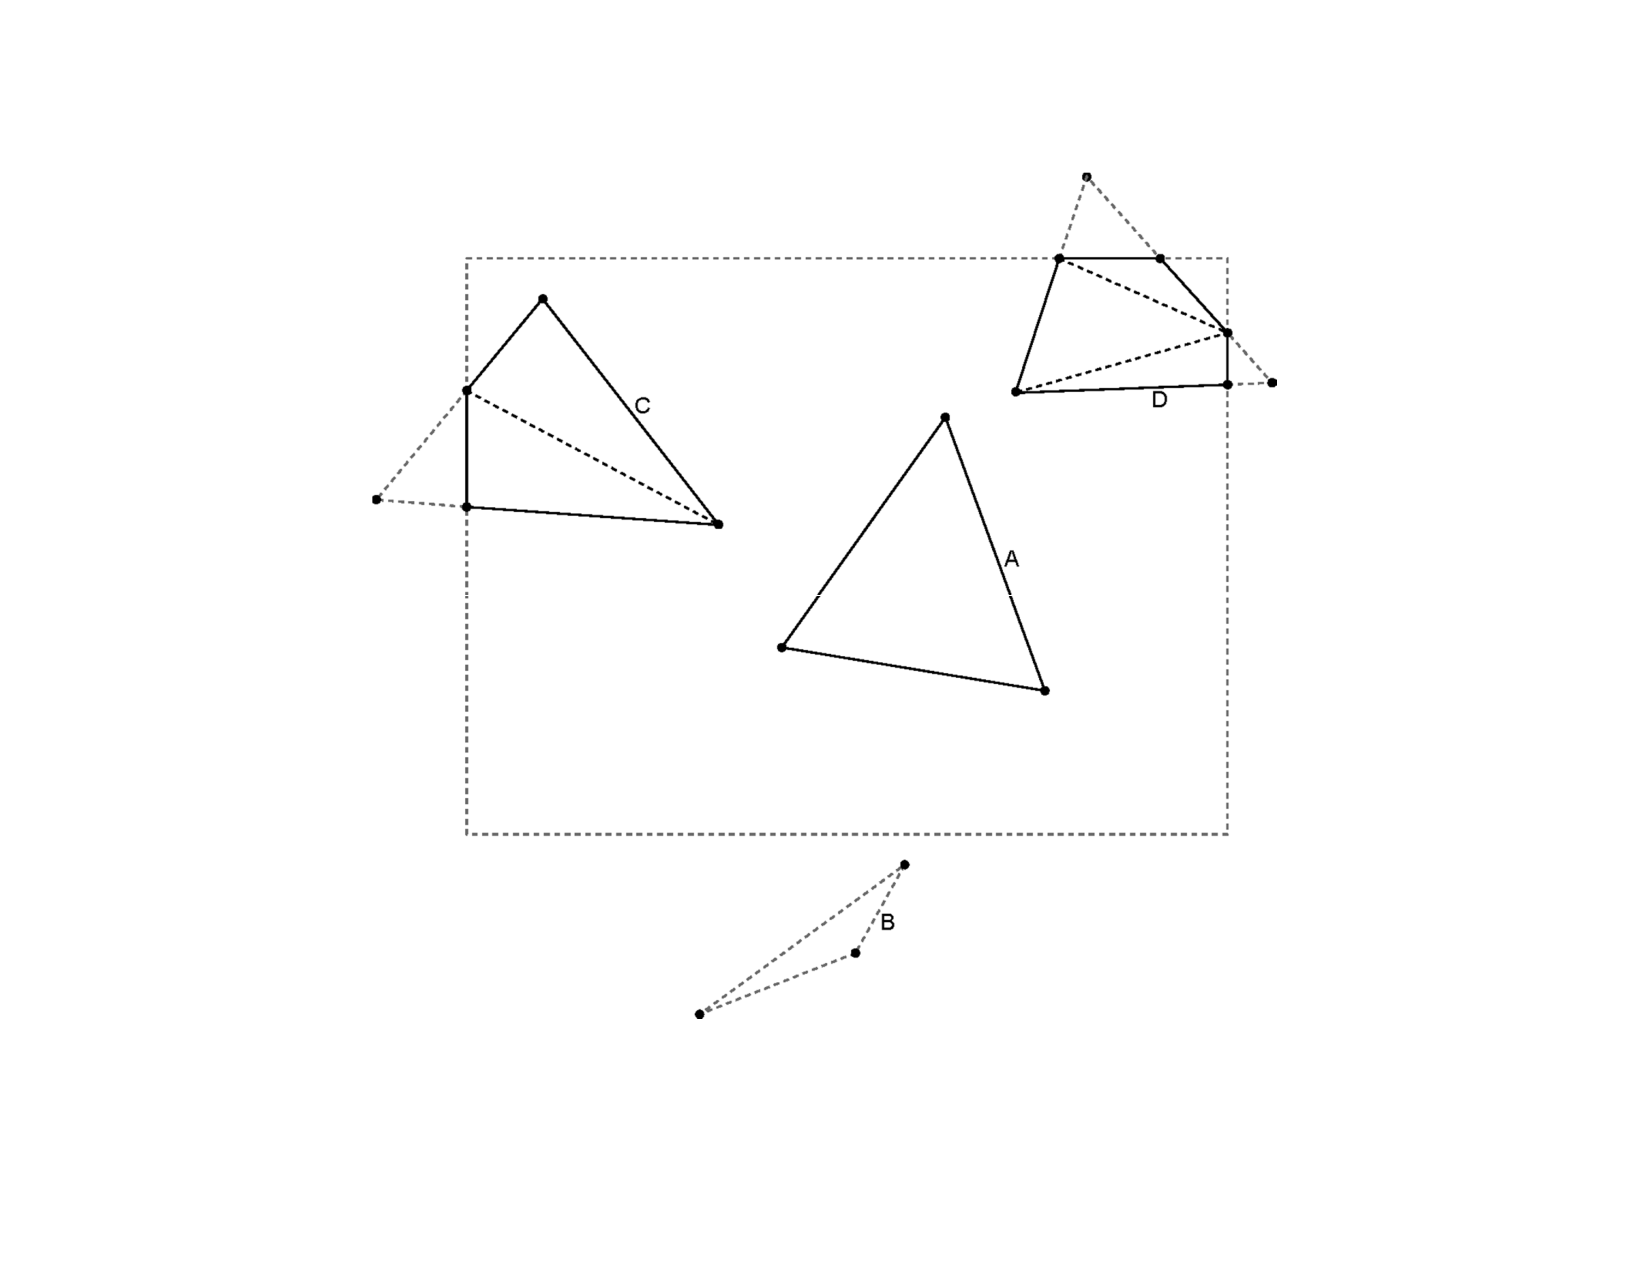
\includegraphics[width=0.35\textwidth]{clip_space}
	\caption{Clip Space \cite{superbible}}
	\label{fig:clip-space}
\end{figure}

To transform vertex coordinates from view to clip-space a \textbf{projection matrix} is defined specifying a range of coordinates. The projection matrix then transforms coordinates within this specified range to \gls{gls-normalized-device-coordinates}. All coordinates outside this range will not be mapped and therefore be clipped \cite{learnopengl}. 


\subsubsection{Orthographic and Perspective Projections} \label{projections}

The \emph{viewing box} product of the \textbf{projection matrix} is also called a \gls{frustum}. Each coordinate that ends up inside the frustum will end up on the user's screen.

\begin{figure}[h!]
	\centering
	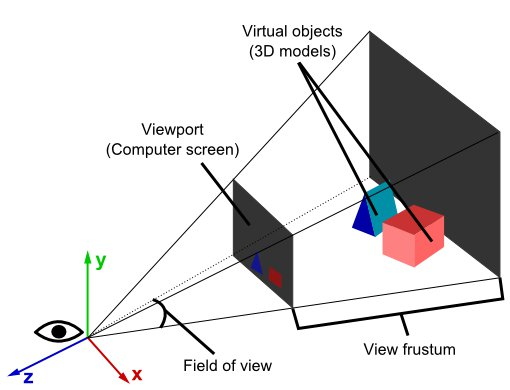
\includegraphics[width=0.35\textwidth]{frustum}
	\caption{Frustum \cite{realtutorials}}
	\label{fig:frustum}
\end{figure}

The process to convert coordinates within a specified range to \gls{NDC} is called \textbf{projection} or \textbf{projection transformation} since the projection matrix projects 3D coordinates to the 2D \gls{gls-normalized-device-coordinates}.\hl {"The projection transformation specifies how a finished scene is projected to the final image on the screen" \cite{superbible}}. 

The projection matrix to transform view coordinates to clip coordinates can take two different forms, where each form defines its own unique frustum. It is possible to either create an \textbf{orthographic projection matrix} or a \textbf{perspective projection matrix}.

\subsubsubsection{Orthographic Projection Matrix}

An orthographic projection matrix defines a cube-like frustum box for the clipping space where each vertex outside this box is discarded. 
When creating an orthographic projection matrix we specify the width, height and length of the visible frustum. All the coordinates which end up inside this frustum after transforming them to clip space with the orthographic projection matrix, will not be clipped and therefore visible on the resulting display. The frustum looks a bit like a container:


\begin{figure}[h!]
	\centering
	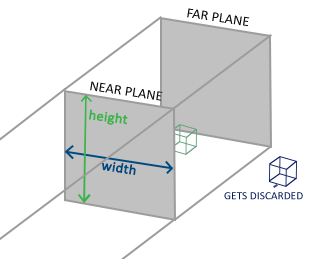
\includegraphics[width=0.35\textwidth]{orthographic_frustum}
	\caption{Orthographic frustum \cite{learnopengl}}
	\label{fig:orthographic_frustum}
\end{figure}

An orthographic projection matrix directly maps coordinates to the 2D plane that is the screen, but in reality a direct projection produces unrealistic results since the projection does not take the perspective into account. 

\subsubsubsection{Perspective Projection Matrix}

The projection matrix maps a given frustum range to clip space too, but also manipulates the \verb|w| value or \emph{homogeneous coordinate} of each vertex coordinate in such a way that the further away a vertex coordinate is from the viewer, the higher this \verb|w| component becomes. This makes distant objects appear smaller than nearby objects of the same size:


\begin{figure}[h!]
	\centering
	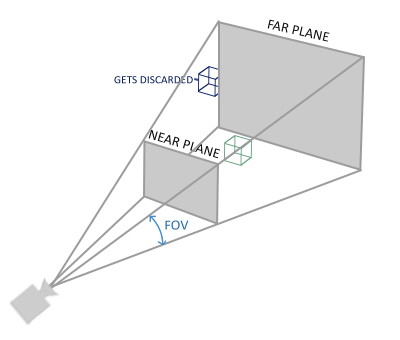
\includegraphics[width=0.4\textwidth]{perspective_frustum}
	\caption{Perspective frustum \cite{learnopengl}}
	\label{fig:perspective_frustum}
\end{figure}

A comparison of both perspectives:

\begin{figure}[h!]
	\centering
	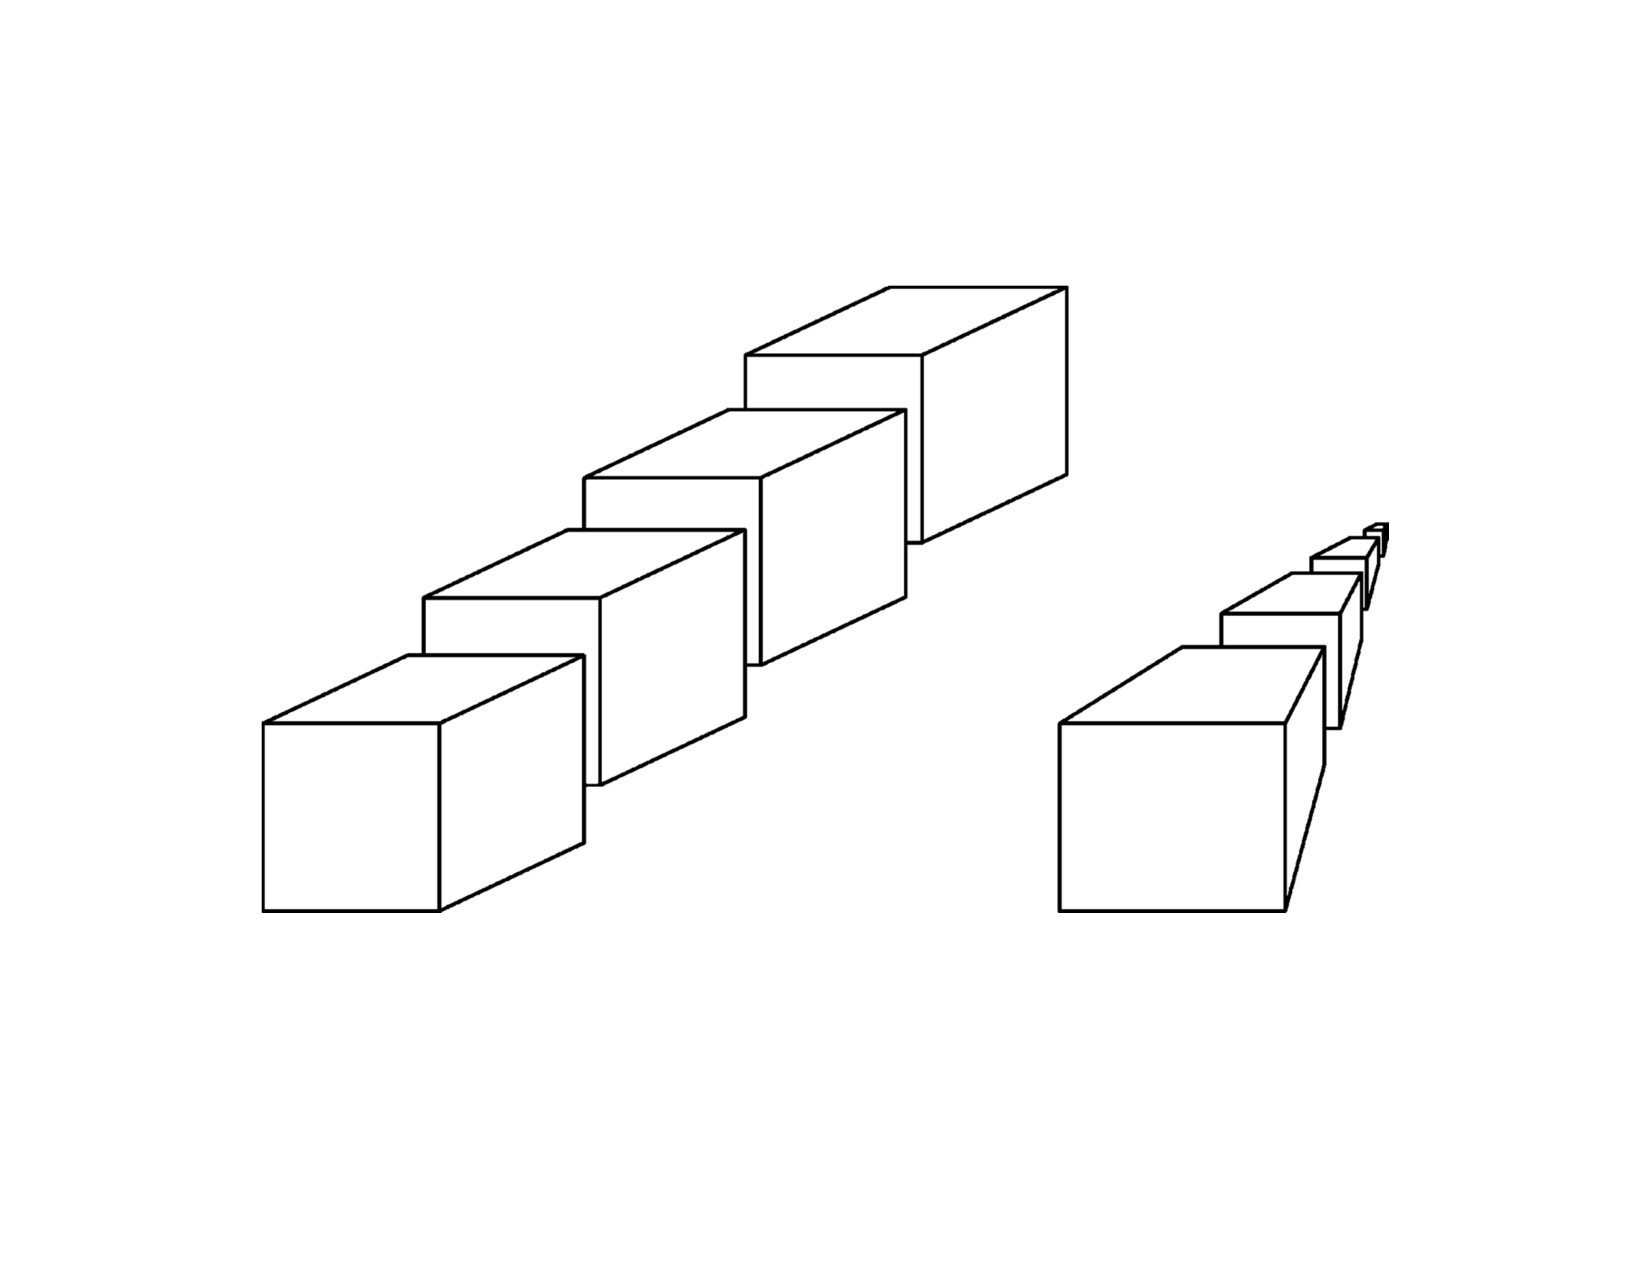
\includegraphics[width=0.35\textwidth]{orthographic_and_perspective_projections}
	\caption{Orthographic and Perspective projections \cite{superbible}}
	\label{fig:orthographic_and_perspective_projections}
\end{figure}

\subsubsection{Spaces and Transformations summary}

In the figure \ref{fig:coordinate_systems} we can observe all the transformations or steps needed to display an object or model from its \glspl{vertex} to the screen:

\begin{figure}[h!]
	\centering
	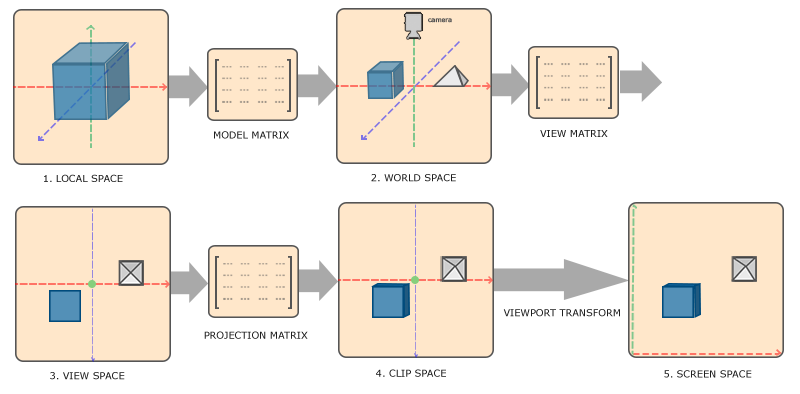
\includegraphics[width=0.9\textwidth]{coordinate_systems}
	\caption{Coordinate systems \cite{learnopengl}}
	\label{fig:coordinate_systems}
\end{figure}

\subsubsection{Camera}
In \gls{opengl} there is no concept of a \emph{camera} as in the video game world. Usually a camera simulation is created \hl{"by moving all objects in the scene in the reverse direction"}, giving the illusion that the observer is moving \cite{learnopengl} when instead the objects are just rearranged.

In the \gls{view-space} the vertex coordinates are seen from the camera's perspective, i.e, the camera perspective seems to be the origin of the scene. \newline
In order to define a camera, the following points need to be known or identified: 
\begin{itemize}
	\item the camera's position in world space
	\item the direction the camera is facing
	\item a vector pointing to the right of the camera
	\item a vector pointing upwards from the camera
\end{itemize} 
This process of forming the view / camera space coordinates system is known as the Gram-Schmidt process \cite{gramprocess} in linear algebra and creates a coordinate system with the camera's position as the origin:
\begin{figure}[h!]
	\centering
	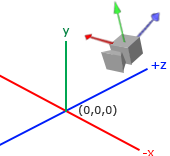
\includegraphics[width=0.3\textwidth]{camera_axes}
	\caption{Camera as coordinate system \cite{cameraopengl}}
	\label{fig:camera-opengl}
\end{figure}

\subsubsubsection{Camera Position}

\hl{"The camera position is basically a vector in world space that points to the camera's position" \cite{cameraopengl}}.
As you can observe in Figure \ref{fig:camera-opengl}, the positive $z-axis$ goes through the screen towards the user. As a result, movement along the $z-axis$ will result in a forward/backward movement of the camera in this case.

\subsubsubsection{Camera Direction}

Or at what direction is the camera pointing at. If we point the camera to the scene origin $(0, 0, 0)$, the direction vector will be the result of subtracting the camera position vector form the scene's origin vector.

\subsubsubsection{Camera Right Axis}

This vector can either be specified yourself (typically: $(1, 0, 0)$) or calculated based on the \emph{up-vector} that points upwards in world space.

\centerline{$cameraRight = cameraUp \times cameraDirection$}

The calculation is using the cross product of the \emph{up-vector} and the \emph{direction-vector}. Since the result of a cross product is a vector perpendicular to both vectors, we will get a vector that points towards the right from the camera's point of view (PoV).

\subsubsubsection{Camera Up Axis}

This vector can also either be specified yourself (typically: $(0, 1, 0)$) or calculated based on the \emph{right-vector} that points towards the right from the camera's position. 

\centerline{$cameraUp = cameraRight \times cameraDirection$}

\subsubsubsection{LookAt Matrix}

The \emph{LookAt matrix} is defined with the three camera axes plus a translation vector. With it you can transform any vector to that coordinate space by multiplying it with this matrix:

\centerline{
$LookAt = 
\begin{bmatrix} \color{red}{R_x} & \color{red}{R_y} & \color{red}{R_z} & 0 \\ 
				\color{green}{U_x} & \color{green}{U_y} & \color{green}{U_z} & 0 \\ 
				\color{blue}{D_x} & \color{blue}{D_y} & \color{blue}{D_z} & 0 \\ 
				0 & 0 & 0  & 1 \end{bmatrix} 
				* \begin{bmatrix} 1 & 0 & 0 & -\color{purple}{P_x} \\ 
				0 & 1 & 0 & -\color{purple}{P_y} \\ 
				0 & 0 & 1 & -\color{purple}{P_z} \\ 
				0 & 0 & 0  & 1 \end{bmatrix}$ }

Where {\color{red}R} is the right vector, {\color{green}U} is the up vector, {\color{blue}D} is the direction vector and {\color{purple}P} is the camera's position vector. Note that the position vector is inverted since we eventually want to translate the world in the opposite direction of where we want to move. 


\hl{"Using this \emph{LookAt matrix} as our view matrix effectively transforms all the world coordinates to the view space we just defined. The LookAt matrix then does exactly what it says: It creates a view matrix that looks at a given target" \cite{cameraopengl}.}

The GLM library \cite{glm} provides a \verb|glm::lookAt| function. It is only necessary to specify a camera position, a target position and a vector that represents the up vector in world space. GLM then creates the LookAt matrix that can be used as the \ref{view-matrix} View Matrix using the process described above:


\begin{lstlisting}[language=C++, caption={GLM lookAt function example}, label={code:lookat}]
glm::mat4 view;
view = glm::lookAt(glm::vec3(0.0f, 0.0f, 3.0f), 
		glm::vec3(0.0f, 0.0f, 0.0f), 
		glm::vec3(0.0f, 1.0f, 0.0f));
\end{lstlisting}


\subsubsection{Lighting}

\hl{"Lighting in \gls{opengl} is based on approximations of reality using models that are much easier to process than reality and look relatively similar" \cite{lightinglearnopengl}.} One of these models is the \gls{phong} and it consists of the following three components: \emph{ambient}, \emph{diffuse} and \emph{specular} lighting.

\subsubsubsection{Ambient Lighting}

\hl{"Light in a scene that doesn't come from any specific point source or direction. Ambient light illuminates all surfaces evenly and on all sides" \cite{superbible}.} To simulate this an ambient lighting constant that always gives the objects some colour is used. This constant is added to the final resulting colour of the object's \gls{fragment-shader}, thus making it look like there always is some scattered light even when there is no a direct source of light.

\subsubsubsection{Diffuse Lighting}

\hl{"Diffuse light is the directional component of a light source"} \cite{superbible} and simulates the directional impact a light object has on an object. This is the most visually significant component of the lighting model. The more a part of an object faces the light source, the brighter it becomes.


\begin{figure}[h!]
	\centering
	
\includegraphics[width=0.4\textwidth]{diffuse_light}
	\caption{Diffuse Light \cite{lightinglearnopengl}}
	\label{fig:diffuse-light}
\end{figure}

In the figure \ref{fig:diffuse-light} we can see a light source on the left with a light ray pointing towards the object. It is necessary to measure at what angle the light ray touches the fragment. 

If the light ray is perpendicular to the object's surface the light has the greatest impact. To measure the angle between the light ray and the fragment we use a normal vector $\overrightarrow{N}$ \cite{normalvector} to the fragment's surface. The angle between the two vectors can then easily be calculated using the dot product.

So, the resulting dot product returns a scalar that can be used to calculate the light's impact on the fragment's colour, resulting in fragments with different lighting/illumination, based on their orientation towards the light.

Therefore, in order to calculate diffuse lighting the following factors are needed \cite{lightinglearnopengl}: 
\begin{itemize}
	\item Normal vector $\overrightarrow{N}$: a vector perpendicular to the vertex' surface.
	\item The directed light ray: a direction vector, which is the result of the subtraction of the light's position from the fragment's position. Therefore we need both the light's position vector and the fragment's position vector for our calculation.
\end{itemize}


\subsubsubsection{Specular Lighting}

\hl{"Specular light is a highly directional property, but it interacts more sharply with the surface and in a particular direction" \cite{superbible},} f.e. from what direction the user is looking at the fragment.

A highly specular light tends to cause a bright spot on the surface it shines on, which is called the \emph{\hl{"specular highlight"}} \cite{superbible}. Specular highlights are often more inclined to the colour of the light than the colour of the object.


\begin{figure}[h!]
	\centering
	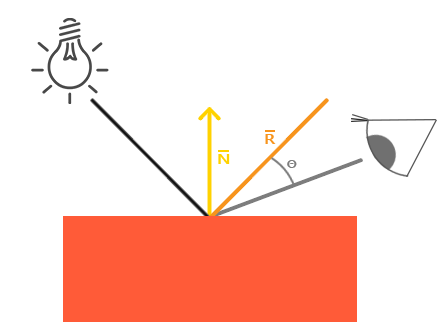
\includegraphics[width=0.4\textwidth]{specular_lighting}
	\caption{Specular Lighting \cite{lightinglearnopengl}}
	\label{fig:specular-lighting}
\end{figure}


We calculate a reflection vector $\overrightarrow{R}$ by reflecting the light direction around the normal vector $\overrightarrow{N}$. Then we calculate the angular distance between this reflection vector and the view direction. The closer the angle $\Theta$ between them, the greater the impact of the specular light. The resulting effect is the bright spot when we're looking at the light's direction reflected via the object.

The view vector is the one extra variable needed for specular lighting which can be calculated using the viewer's world space position and the fragment's position. 
Then we calculate the specular light's intensity, multiply this with the light colour and add this to the resulting ambient and diffuse components.\cite{lightinglearnopengl}

In the Figure \ref{fig:basic_lighting_phong} you can see what the different lighting components might look like: 

\begin{figure}[h!]
	\centering
	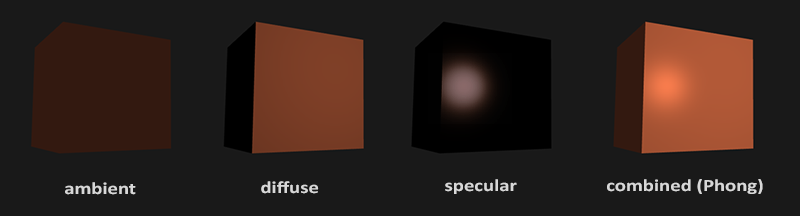
\includegraphics[width=0.6\textwidth]{basic_lighting_phong}
	\caption{Lighting Components \cite{lightinglearnopengl}}
	\label{fig:basic_lighting_phong}
\end{figure}

